\documentclass[12pt, unicode, svgnames, handout]{beamer}

\definecolor{links}{HTML}{2A1B81}
\hypersetup{colorlinks,linkcolor=,urlcolor=links}

\usetheme{Boadilla}
\usecolortheme{seahorse}
\usefonttheme{serif}
\beamertemplatenavigationsymbolsempty

\usepackage{luatexja}
\usepackage{pgfpages}
\usepackage[hiragino-pro, deluxe, expert]{luatexja-preset}
\usepackage[osf]{mathpazo}
\usepackage{fontspec}
\usepackage{epigraph}
\usepackage{ifxetex,ifluatex}
\usepackage{etoolbox}
\usepackage{tikz}
\usepackage{framed}
\usepackage{libertine}
\usepackage[final]{listings}
\usepackage{amsmath}
\usepackage{pgf-umlsd}
\usepackage{mathtools}

%\setbeameroption{show notes on second screen=right}

\usetikzlibrary{arrows,automata,shapes,backgrounds}

\setmainfont[Numbers=OldStyle, BoldFont=Palatino Bold]{Palatino}
\setsansfont{CMU Sans Serif}
\setmonofont{CMU Typewriter Text}
\setmainjfont[BoldFont=Hiragino Kaku Gothic Pro W6]{Hiragino Kaku Gothic Pro W3}

\title[Regular expressions à la carte]{%
  \href{https://github.com/y-yu/regex-slide}{Regular expressions à la carte} \\
  \href{http://kbkz.connpass.com/event/26677/}{\normalsize kbkz.tech \#9}
}
\author{吉村 優}
\date{March 20, 2016}
\institute[\url{https://twitter.com/\_yyu\_}]{%
  \url{https://twitter.com/\_yyu\_}\\
  \url{http://qiita.com/yyu}\\
  \url{https://github.com/y-yu}\\
}

\input{./lib/ballon.tex}
\input{./lib/quotebox.tex}
\newfontfamily\listingfont{Consolas}

\lstset{
  basicstyle=\listingfont
}

\lstdefinestyle{cpp}{
  basicstyle=\listingfont\footnotesize,        % the size of the fonts that are used for the code
  breakatwhitespace=false,         % sets if automatic breaks should only happen at whitespace
  language=C++,
  firstnumber=0,
  xleftmargin=2em,
  framexleftmargin=1.5em,
  numberstyle=\listingfont\scriptsize,
  breaklines=true,                 % sets automatic line breaking
  captionpos=b,                    % sets the caption-position to bottom
  commentstyle=\listingfont\color{green},    % comment style
  extendedchars=true,              % lets you use non-ASCII characters; for 8-bits encodings only, does not work with UTF-8
  keepspaces=true,                 % keeps spaces in text, useful for keeping indentation of code (possibly needs columns=flexible)
  keywordstyle=\listingfont\color{blue},       % keyword style
  rulecolor=\listingfont\color{black},         % if not set, the frame-color may be changed on line-breaks within not-black text (e.g. comments (green here))
  showspaces=false,                % show spaces everywhere adding particular underscores; it overrides 'showstringspaces'
  showstringspaces=false,          % underline spaces within strings only
  showtabs=false,                  % show tabs within strings adding particular underscores
  showlines=false,
  stringstyle=\listingfont\color{gray},        % string literal style
  tabsize=2,	                   % sets default tabsize to 2 spaces
  title=\lstname                   % show the filename of files included with \lstinputlisting; also try caption instead of title
}

\lstdefinestyle{vm}{
  basicstyle=\listingfont\footnotesize,        % the size of the fonts that are used for the code
  breakatwhitespace=false,         % sets if automatic breaks should only happen at whitespace
  morekeywords={char,split,jmp,match},
  numbers=left,
  firstnumber=0,
  xleftmargin=2em,
  framexleftmargin=1.5em,
  numberstyle=\listingfont\scriptsize,
  breaklines=true,                 % sets automatic line breaking
  captionpos=b,                    % sets the caption-position to bottom
  commentstyle=\listingfont\color{green},    % comment style
  extendedchars=true,              % lets you use non-ASCII characters; for 8-bits encodings only, does not work with UTF-8
  keepspaces=true,                 % keeps spaces in text, useful for keeping indentation of code (possibly needs columns=flexible)
  keywordstyle=\listingfont\color{blue},       % keyword style
  rulecolor=\listingfont\color{black},         % if not set, the frame-color may be changed on line-breaks within not-black text (e.g. comments (green here))
  showspaces=false,                % show spaces everywhere adding particular underscores; it overrides 'showstringspaces'
  showstringspaces=false,          % underline spaces within strings only
  showtabs=false,                  % show tabs within strings adding particular underscores
  showlines=false,
  stringstyle=\listingfont\color{gray},        % string literal style
  tabsize=2,	                   % sets default tabsize to 2 spaces
  title=\lstname                   % show the filename of files included with \lstinputlisting; also try caption instead of title
}

\lstdefinestyle{grass}{
  basicstyle=\listingfont\scriptsize,        % the size of the fonts that are used for the code
  breakatwhitespace=false,         % sets if automatic breaks should only happen at whitespace
  xleftmargin=2em,
  framexleftmargin=1.5em,
  numberstyle=\listingfont\scriptsize,
  breaklines=true,                 % sets automatic line breaking
  captionpos=b,                    % sets the caption-position to bottom
  commentstyle=\listingfont\color{green},    % comment style
  extendedchars=true,              % lets you use non-ASCII characters; for 8-bits encodings only, does not work with UTF-8
  keepspaces=true,                 % keeps spaces in text, useful for keeping indentation of code (possibly needs columns=flexible)
  keywordstyle=\listingfont\color{blue},       % keyword style
  rulecolor=\listingfont\color{black},         % if not set, the frame-color may be changed on line-breaks within not-black text (e.g. comments (green here))
  showspaces=false,                % show spaces everywhere adding particular underscores; it overrides 'showstringspaces'
  showstringspaces=false,          % underline spaces within strings only
  showtabs=false,                  % show tabs within strings adding particular underscores
  showlines=false,
  stringstyle=\listingfont\color{gray},        % string literal style
  tabsize=2,	                   % sets default tabsize to 2 spaces
  title=\lstname                   % show the filename of files included with \lstinputlisting; also try caption instead of title
}


\input{./lib/footnotemark.tex}
\input{./lib/mydescription.tex}

\newcommand\ballref[1]{%
\tikz \node[circle, shade,ball color=structure.fg,inner sep=0pt,%
  text width=8pt,font=\tiny,align=center] {\color{white}\ref{#1}};
}

%\everymath{\displaystyle}

\begin{document}

\frame{\maketitle}

\section{自己紹介}
\begin{frame}[fragile]
  \frametitle{自己紹介}
  
  \begin{columns}
    \begin{column}{0.3\textwidth}
      \centering
      \begin{figure}
        \includegraphics[width=.7\textwidth]{img/bird2x.png}
      \end{figure}
    \end{column}
    \begin{column}{0.7\textwidth}
      \begin{Ldescription}
        \small
        \item<2->[VM型の正規表現エンジンを実装する]
          \url{http://qiita.com/yyu/items/84b1a00459408d1a7321}
        \item<3->[正規表現からLLVMへのコンパイラを実装する]
          \url{http://qiita.com/yyu/items/a0ef2d2204c137707f3f}
        \item<4->[正規表現のJITコンパイラを実装する]
          \url{http://qiita.com/yyu/items/3c4deb39d6b0a7955572}
        \item<5->[正規表現の微分でサブマッチング]
          \url{http://qiita.com/yyu/items/1638fd59bedce27ca3a4}
      \end{Ldescription}
    \end{column}
  \end{columns}
\end{frame}

\section*{アウトライン}
\begin{frame}[fragile]
  \frametitle{アウトライン}

  \begin{enumerate}
    \item<2-> 正規表現とは?
    \item<3-> マッチング
    \item<4-> 正規表現の限界
    \item<5-> 正規表現 vs C++
  \end{enumerate}
\end{frame}

\section{正規表現とは?}
\begin{frame}[fragile]
  \frametitle{正規表現とは?}

  \uncover<2->{
    \begin{block}{}
      \begin{shadequote}[r]{\scriptsize\href{https://ja.wikipedia.org/wiki/\%E6\%AD\%A3\%E8\%A6\%8F\%E8\%A1\%A8\%E7\%8F\%BE}{Wikipedia - 正規表現}}
        \textbf{正規表現}とは、文字列の集合を一つの文字列で表現する方法の一つである。
      \end{shadequote}
    \end{block}
  }

  \uncover<3->{
    \begin{block}{}
      \begin{shadequote}[r]{\scriptsize\href{https://ja.wikipedia.org/wiki/\%E6\%AD\%A3\%E8\%A6\%8F\%E8\%A1\%A8\%E7\%8F\%BE}{Wikipedia - 正規表現}}
        もともと正規表現は形式言語理論において正規言語を表すための手段として導入された。
      \end{shadequote}
    \end{block}
  }
\end{frame}

\subsection{正規言語}
\begin{frame}[fragile]
  \frametitle{正規言語}

  \begin{block}{}
    \begin{shadequote}[r]{\scriptsize\href{https://ja.wikipedia.org/wiki/\%E6\%AD\%A3\%E8\%A6\%8F\%E8\%A8\%80\%E8\%AA\%9E}{Wikipedia - 正規言語}}
      \textbf{正規言語}とは、以下に示す性質を満たす形式言語のことである。
      \begin{itemize}
        \item<2-> 正規表現で記述可能
        \item<3-> 非決定性有限オートマトン(NFA)で受理可能
        \item<4-> 決定性有限オートマトン(DFA)で受理可能
      \end{itemize}
    \end{shadequote}
  \end{block}
\end{frame}

\begin{frame}[fragile]
  \frametitle{正規表現の定義}

  文字の集合$\Sigma$上の正規表現は次のように定義される
  \begin{block}{}
    \begin{itemize}
      \item<2-> 空集合を表す$\phi$は正規表現
      \item<3-> 空文字を表す$\epsilon$は正規表現
      \item<4-> $a \in \Sigma$は正規表現
      \item<5-> $X$と$Y$が正規表現であるとき次のものも正規表現
        \begin{itemize}
          \item<6-> $X \mid Y$(選択)
          \item<7-> $X Y$(結合)
          \item<8-> $X^*$(0回以上の繰り返し)
        \end{itemize}
    \end{itemize}
  \end{block}
\end{frame}

\section{マッチング}
\begin{frame}[fragile]
  \frametitle{マッチング}

  主に次のような方法がある
  \begin{itemize}
    \item<2-> 有限オートマトンを用いた方法
    \item<3-> Virtual Machineを用いた方法
    \item<4-> 正規表現の微分を用いた方法
  \end{itemize}
\end{frame}

\subsection{NFAを用いたマッチング}
\begin{frame}[fragile]
  \frametitle{非決定性有限オートマトン(NFA)}
  
  \begin{block}{}
    \begin{shadequote}[r]{\scriptsize\href{https://ja.wikipedia.org/wiki/\%E9\%9D\%9E\%E6\%B1\%BA\%E5\%AE\%9A\%E6\%80\%A7\%E6\%9C\%89\%E9\%99\%90\%E3\%82\%AA\%E3\%83\%BC\%E3\%83\%88\%E3\%83\%9E\%E3\%83\%88\%E3\%83\%B3}{Wikipedia - 非決定性有限オートマトン}}
      \textbf{非決定性有限オートマトン}は、有限オートマトンの一種であり、ある状態と入力があったとき、次の遷移先が一意に決定しないことがあるものである。
    \end{shadequote}
  \end{block}

  \uncover<2->{
    \begin{center}
      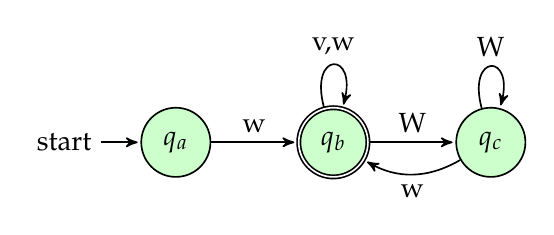
\begin{tikzpicture}[->,>=stealth',shorten >=1pt,auto,node distance=2cm,semithick]
        \tikzstyle{every state}=[fill=green!20, text=black]
      
        \node[initial,state]     (A)                          {$q_a$};
        \node[accepting,state]   (B)       [right of=A]       {$q_b$};
        \node[state]             (C)       [right of=B]       {$q_c$};
      
        \path (A) edge              node {w}     (B)
              (B) edge [loop above] node {v,w}   (B)
                  edge              node {W}     (C)
              (C) edge [bend left]  node {w}     (B)
                  edge [loop above] node {W}     (C);
      \end{tikzpicture}
    \end{center}
  }
\end{frame}

\begin{frame}[fragile]
  \frametitle{NFAを用いたマッチング}

  \begin{itemize}
    \item 全ての正規表現には対応する非決定性有限オートマトンが存在する
  \end{itemize}
\end{frame}

\begin{frame}[fragile]
  \frametitle{正規表現とNFA}

  \begin{Ldescription}
    \item<1->[文字$N(a)$]
      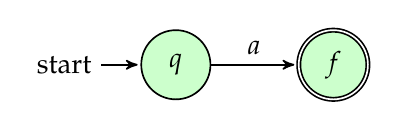
\begin{tikzpicture}[->,>=stealth',shorten >=1pt,auto,node distance=2cm,semithick]
        \tikzstyle{every state}=[fill=green!20, text=black]
      
        \node[initial,state]     (A)                          {$q$};
        \node[accepting,state]   (B)       [right of=A]       {$f$};
      
        \path (A) edge node {$a$} (B);
      \end{tikzpicture}

    \item<2->[選択$N(s \mid t)$]
      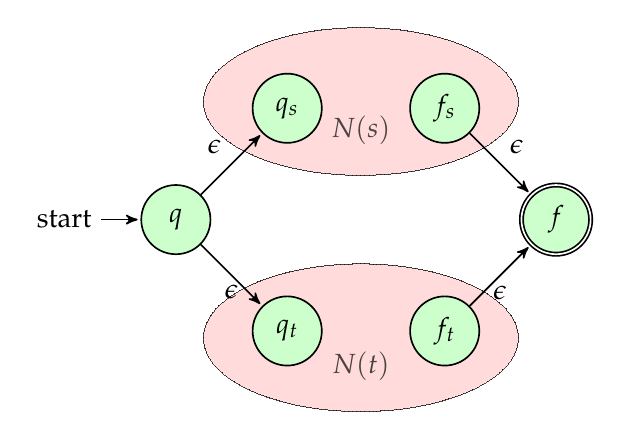
\begin{tikzpicture}[->,>=stealth',shorten >=1pt,auto,node distance=2cm,semithick]
        \tikzstyle{every state}=[fill=green!20, text=black]
      
        \node[ellipse, draw, line width=0mm, fill=red!20, opacity=.7, text height =1cm, minimum width = 4cm] at (2.35,1.5) {$N(s)$};
        \node[ellipse, draw, line width=0mm, fill=red!20, opacity=.7, text height =1cm, minimum width = 4cm] at (2.35,-1.5) {$N(t)$};
        \node[initial,state]     (A)                                {$q$};
        \node[state]             (B)       [above right of=A]       {$q_s$};
        \node[state]             (C)       [below right of=A]       {$q_t$};
        \node[state]             (D)       [right of=B]             {$f_s$};
        \node[state]             (E)       [right of=C]             {$f_t$};
        \node[accepting, state]  (F)       [below right of=D]       {$f$};


        \path (A) edge node         {$\epsilon$} (B)
                  edge node [below] {$\epsilon$} (C)
              (D) edge node         {$\epsilon$} (F)
              (E) edge node [below] {$\epsilon$} (F);
      \end{tikzpicture}
  \end{Ldescription}
\end{frame}

\begin{frame}[fragile]
  \frametitle{正規表現とNFA}

  \begin{Ldescription}
    \item<1->[結合$N(st)$]
      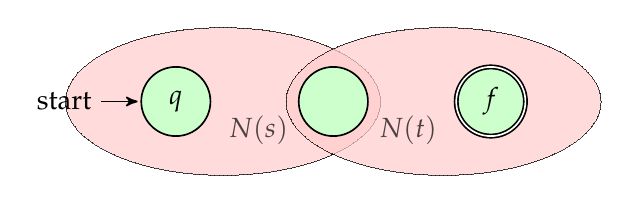
\begin{tikzpicture}[->,>=stealth',shorten >=1pt,auto,node distance=2cm,semithick]
        \tikzstyle{every state}=[fill=green!20, text=black]
      
        \node[ellipse, draw, line width=0mm, fill=red!20, opacity=.7, text height =1cm, minimum width = 4cm] at (0.6,0) {$\hspace{0.9cm} N(s)$};
        \node[ellipse, draw, line width=0mm, fill=red!20, opacity=.7, text height =1cm, minimum width = 4cm] at (3.4,0) {$N(t) \hspace{0.9cm}$};
        \node[initial,state]     (A)                          {$q$};
        \node[state]             (B)       [right of=A]       {};
        \node[accepting,state]   (C)       [right of=B]       {$f$};
      
      \end{tikzpicture}

    \item<2->[繰り返し$N(s^*)$]
      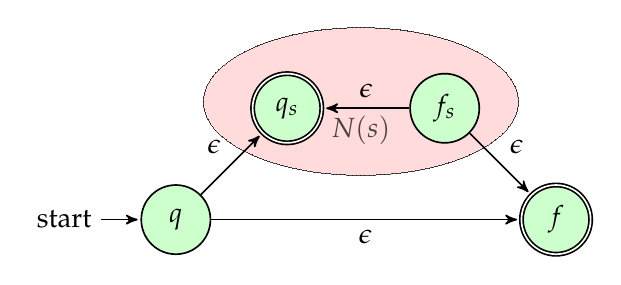
\begin{tikzpicture}[->,>=stealth',shorten >=1pt,auto,node distance=2cm,semithick]
        \tikzstyle{every state}=[fill=green!20, text=black]
      
        \node[ellipse, draw, line width=0mm, fill=red!20, opacity=.7, text height =1cm, minimum width = 4cm] at (2.35,1.5) {$N(s)$};
        \node[initial,state]     (A)                          {$q$};
        \node[accepting, state]  (B)       [above right of=A] {$q_s$};
        \node[state]             (C)       [right of=B]       {$f_s$};
        \node[accepting, state]  (D)       [below right of=C] {$f$};


        \path (A) edge node          {$\epsilon$} (B)
                  edge node [below]  {$\epsilon$} (D)
              (C) edge node          {$\epsilon$} (D)
                  edge node [above]  {$\epsilon$} (B); 
      \end{tikzpicture}
  \end{Ldescription}
\end{frame}

\begin{frame}[fragile]
  \frametitle{NFAを用いたマッチング}

  \begin{itemize}
    \item 全ての正規表現には対応する非決定性有限オートマトンが存在する
    \item 遷移先が一意に決まらないので、バックトラックをする必要がある
  \end{itemize}
\end{frame}

\subsection{DFAを用いたマッチング}
\begin{frame}[fragile]
  \frametitle{決定性有限オートマトン(DFA)}
  
  \begin{block}{}
    \begin{shadequote}[r]{\scriptsize\href{https://ja.wikipedia.org/wiki/\%E5\%B1\%BA\%E5\%AE\%9A\%E6\%80\%A7\%E6\%9C\%89\%E9\%99\%90\%E3\%82\%AA\%E3\%83\%BC\%E3\%83\%88\%E3\%83\%9E\%E3\%83\%88\%E3\%83\%B3}{Wikipedia - 決定性有限オートマトン}}
      \textbf{決定性有限オートマトン}は、状態と入力によって次に遷移すべき状態が一意に定まる有限オートマトンである。
    \end{shadequote}
  \end{block}

  \uncover<2->{
    \begin{center}
      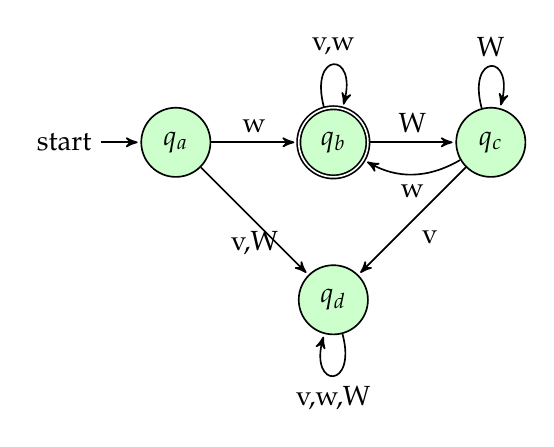
\begin{tikzpicture}[->,>=stealth',shorten >=1pt,auto,node distance=2cm,semithick]
        \tikzstyle{every state}=[fill=green!20, text=black]
      
        \node[initial,state]     (A)                          {$q_a$};
        \node[accepting,state]   (B)       [right of=A]       {$q_b$};
        \node[state]             (C)       [right of=B]       {$q_c$};
        \node[state]             (D)       [below of=B]       {$q_d$};
      
        \path (A) edge              node {w}     (B)
                  edge [below]      node {v,W}   (D)
              (B) edge [loop above] node {v,w}   (B)
                  edge              node {W}     (C)
              (C) edge [bend left]  node {w}     (B)
                  edge [loop above] node {W}     (C)
                  edge              node {v}     (D)
              (D) edge [loop below] node {v,w,W} (D);
      \end{tikzpicture}
    \end{center}
  }
\end{frame}

\begin{frame}[fragile]
  \frametitle{DFAを用いたマッチング}
  
  \begin{itemize}
    \item<1-> 非決定性有限オートマトンから機械的に変換できる(サブセット構成など)
    \item<2-> 入力によって状態が一意に決まるので、バックトラックをする必要がない
    \item<3-> 非決定有限オートマトンから変換すると、最悪の場合、\textbf{状態数が指数関数的に増加する}
    \item<4-> そのため、必要になった状態だけ変換するというテクニックがある
  \end{itemize}
\end{frame}

\subsection{VMを用いたマッチング}
\begin{frame}[fragile]
  \frametitle{Virtual Machine(VM)を使ったマッチング}

  \uncover<2->{次のようなVMを用いて正規表現のマッチングが可能}

  \begin{itemize}
    \item<3-> \texttt{PC}と\texttt{SP}という2つのレジスタがある
    \item<4-> 次の命令がある
      \begin{Ldescription}
        \item<5->[\texttt{char c}] \texttt{SP}の先頭の文字と\texttt{c}を比較
        \item<6->[\texttt{match}] マッチに成功(スレッドを終了)
        \item<7->[\texttt{jmp x}] アドレス\texttt{x}へジャンプ(\texttt{PC}を\texttt{x}にする)
        \item<8->[\texttt{split x, y}] スレッドを二つに分割する。
          片方は\texttt{PC}を\texttt{x}にし、もう片方は\texttt{PC}を\texttt{y}にする
      \end{Ldescription}
  \end{itemize}
\end{frame}

\begin{frame}[fragile]
  \frametitle{Virtual Machine(VM)を用いたマッチング}

  正規表現を次のように変換する

  \begin{center}
    \begin{columns}
      \begin{column}{0.4\textwidth}
        \begin{Ldescription}
          \item<2->[文字($c$)]
            \begin{tabular}{l}
              \texttt{char } $c$ \\
            \end{tabular}

          \item<4->[選択($e_1 \mid e_2$)]
            \begin{tabular}{cl}
                     & \texttt{split} $L_1\, L_2$  \\
              $L_1:$ & $e_1$の命令列 \\
                     & \texttt{jmp} $L_3$ \\
              $L_2:$ & $e_2$の命令列 \\
              $L_3:$ & \\
            \end{tabular}
        \end{Ldescription}
      \end{column}
      \begin{column}{0.4\textwidth}
        \begin{Ldescription}
          \item<3->[連結($e_1e_2$)]
            \begin{tabular}{l}
              $e_1$の命令列 \\
              $e_2$の命令列 \\
            \end{tabular}

          \item<5->[繰り返し($e*$)]
            \begin{tabular}{cl}
              $L_1:$ & \texttt{split} $L_1\, L_3$  \\
              $L_2:$ & $e_2$の命令列 \\
                     & \texttt{jmp} $L_1$ \\
              $L_3:$ & \\
            \end{tabular}
        \end{Ldescription}
      \end{column}
    \end{columns}
  \end{center}
\end{frame}

\begin{frame}[fragile]
  \frametitle{Virtual Machine(VM)を用いたマッチング}

  正規表現\lstinline|/aa*bb*/|をVMのバイトコードへ変換する
  
  \begin{exampleblock}{}
    \begin{center}
\begin{lstlisting}[style=vm]
    char a
    split 2, 4
    char a
    jmp 1
    char b
    split 6, 8
    char b
    jmp 5
    match
\end{lstlisting}
    \end{center}
  \end{exampleblock}

  \begin{itemize}
    \item<2-> VMの命令をLLVMやJVMに変換すれば、より高速になる
  \end{itemize}
\end{frame}

\subsection{正規表現の微分を用いたマッチング}
\begin{frame}
  \frametitle{正規表現の微分を用いたマッチング}

  \uncover<2->{
    \begin{block}{正規表現の微分}
      $c:wc$という文字列があるとする%
      \footnote[frame]{この文字列$c:wc$は文字$c$が文字列の先頭の1文字で、$cw$は文字列の先頭以外の残りを表す}。
      ある正規表現$r$が文字列$w:wc$にマッチするならば、
      $r$を文字$c$で微分した正規表現$r_c$は文字列$wc$にマッチする。
    \end{block}
  }
  
  \begin{enumerate}
    \item<3-> マッチング対象の文字列から1文字ずつ取り出し、正規表現を微分していく
    \item<4-> 文字列が空になった時に、微分された正規表現が空文字を受理するならばマッチングに成功
  \end{enumerate}
\end{frame}

\section{正規表現の限界}
\begin{frame}[fragile]
  \frametitle{正規表現の限界}

  \begin{block}{}
    \centering
    \LARGE
    \lstinline{/^1?$|^(11+)\1+$/}
  \end{block}
\end{frame}

\begin{frame}[fragile]
  \frametitle{正規表現の限界}

  \begin{block}{1が非素数個ある文字列の正規表現}
    \centering
    \LARGE
    \lstinline{/^1?$|^(11+)\1+$/}
  \end{block}

  \uncover<2->{
    \begin{exampleblock}{例}
      次のような文字列がマッチする
      \begin{itemize}
        \item $\underbrace{1}_{1?}$
        \item $\underbrace{11}_{11+?}\underbrace{11}_{\backslash 1}$
        \item $\underbrace{111}_{11+?}\underbrace{111}_{\backslash 1}\underbrace{111}_{\backslash 1}$
      \end{itemize}
    \end{exampleblock}
  }
\end{frame}

\subsection{正規表現と非正規表現}
\begin{frame}[fragile]
  \frametitle{正規表現と非正規表現}

  \begin{itemize}
    \item<2-> \textbf{ポンピング補題}などを使うと、
      正規表現で表せる集合かどうか証明できる
    \item<3-> たとえば、次のものは\textbf{正規}である
      \begin{itemize}
        \item ある正規表現の補集合を表す正規表現
        \item 先読み
      \end{itemize}
    \item<4-> たとえば、次のものは\textbf{非正規}である
      \begin{itemize}
        \item 後方参照
        \item 再帰
      \end{itemize}
    \item<5-> 非素数にマッチする正規表現は後方参照を用いていたので、
      非正規表現である
    \item<6-> 非正規になると、正規表現が持つよい性質が失われる
  \end{itemize}
\end{frame}

\section{正規表現 vs C++}
\begin{frame}
  \centering
  {\Huge 正規表現 vs C++\footnote[frame]{この内容は新屋さんの成果です}}
\end{frame}

\subsection{C++}
\begin{frame}[fragile]
  \frametitle{Hello, world!}

  \begin{exampleblock}{Hello, world!}
\begin{lstlisting}[style=cpp]
#include <iostream>

int main()
{
    std::cout << "Hello, World!\n";
    return 0;
}
\end{lstlisting}
  \end{exampleblock}

  \begin{itemize}
    \item<2-> \texttt{Hello, world!}を表示するC++のプログラム
    \item<3-> 全体で86 Byte
  \end{itemize}

\end{frame}

\subsection{Grass}
\begin{frame}[fragile]
  \frametitle{Grass}

  \begin{block}{Grass}
    \begin{shadequote}[r]{\scriptsize\href{http://www.blue.sky.or.jp/grass/}{Grass the grass-planting programming language}}
      Grass is a functional grass-planting programming language.
    \end{shadequote}
  \end{block}

  \begin{itemize}
    \item<2-> C++と同じくチューリング完全なプログラム言語
    \item<3-> \texttt{w}と\texttt{W}と\texttt{v}の組み合せでプログラムが記述できる
    \item<4-> 文法が次のように定義される
      \begin{align*}
        app &::= \mathtt{W}^+\, \mathtt{w}^+ \\
        abs &::= \mathtt{w}^+\, app^* \\
        prog &::= abs \mid prog\, \mathtt{v}\, abs \mid prog\, \mathtt{v}\, app^* 
      \end{align*}
    \item<5-> 文法を\textbf{正規表現}で表せる \\
      \lstinline{w+(W+w+)*((vw*)(W+w+)*)*}
  \end{itemize}
\end{frame}

\begin{frame}[fragile]
  \frametitle{Hello, world!}

  \begin{exampleblock}{Hello, world!}
    \begin{shadequote}[r]{\scriptsize\url{http://d.hatena.ne.jp/rst76/20080708/1215507578}}
\begin{lstlisting}[style=grass]
wvwwWWwWWWwvWwwwwWWwWWWwWWWWwWWWWWwWWWWWWwWWWWWWWwWwwwwww
wwwwwwWWWWwWWWWWWWwWWWWWWWWWWWWWWwWWWWWWWWWWWwwWWWWWWWWWW
wwWWWWWWWWWWWWwWWWWWWWWWWwwWWWWWWWWWWwwwwwwWWWWWWWWWWWWWW
WwWWWWWWWWWWWWWWWWWWWWWwWWWWWWWWWWWWWWWWWWwwWWWWWWWWWWWWW
WWWWwwWWWWWWWWWWWWWWWWWwwwwwWWWWWWWWWWWWWWWWWWWWwwWWWWWWW
WWWWWWWWWWWWWWWwWWWWWWWWWWWWWWWWWWWWWWWWWwwwwwwwwwwwwwwww
wwwwwwwwwwWwwwwwwwwwwWWwwwwwwwWWWwwwwwwwWWWWwWWWWWwwwwwww
wWWWWWWwwwwwwwwwwwwwwwwWWWWWWWwwwwwwwwwwwwwwwwwwwwWWWWWWW
WwwwwwwwwwwwwwwwwwwwwwwwwwwwwwwwwwwwwWWWWWWWWWwwwwWWWWWWW
WWWwwwwwwwwwwwWWWWWWWWWWWwwwwwwwWWWWWWWWWWWWwwwwwwwwwwwww
wwwwwWWWWWWWWWWWWWwwwwwwwwwwwwwwwwwwwwwwwww
\end{lstlisting}
    \end{shadequote}
  \end{exampleblock}

  \begin{itemize}
    \item<2-> Grassで\texttt{Hello, world!}を表示するプログラム
    \item<3-> 613 Byte
  \end{itemize}
\end{frame}

\subsection{RANS}
\begin{frame}[fragile]
  \frametitle{RANS}

  \begin{block}{RANS}
    \begin{shadequote}[r]{\scriptsize\url{http://sinya8282.github.io/RANS/}}
      RANS's concept is very simple, just calculates the number from the given string on a regular language.
    \end{shadequote}
  \end{block}

  \uncover<2-> {
    ある文字列が、ある正規表現が表す集合の何番目に位置するのか計算するプログラム
  }
\end{frame}

\begin{frame}[fragile]
  \frametitle{Hello, world!}

  \texttt{Hello, world!}を表示するプログラムは
  \uncover<2->{
    \begin{exampleblock}{}
      206602040924489026801307911538805854455198744538070639182
      690880761572424911476339257257386704995410169812907136566
      327541800453415305636200196255437899960016989064923911660
      800780259871999465815761462533370076235558393587722548474
      1358948834773649859816115717
    \end{exampleblock}
    番目のGrassプログラム
  }

  \begin{itemize}
    \item<3-> バイナリにすれば107 Byte
    \item<4-> C++と比べて21 Byte差
    \item<5-> 正規表現を工夫すれば、もっと小さくなる(かも)
  \end{itemize}
\end{frame}

\section{参考文献}
\begin{frame}
  \frametitle{参考文献}

  \nocite{*}
  \bibliographystyle{jplain}
  \bibliography{ref}
\end{frame}

\begin{frame}
  \tableofcontents
\end{frame}

\begin{frame}
  \centering
  {\Huge Thank you for listening!}
\end{frame}

\section*{付録}

\subsection*{ポンピング補題}
\begin{frame}
  \frametitle{ポンピング補題}

  $L$が正規言語\footnote[frame]{正規表現で表現できる言語であるという意味}であるならば、次が成り立つ。
  \uncover<2->{
    \begin{block}{}
      任意の正規言語$L$について、言語$L$についてのみ依存する反復長$l > 0$が存在し、
      $|w| \ge l$となる全ての$w \in L$について次が成り立つ
      \begin{enumerate}
        \item
          $|y| > 0$かつ$|xy| \le l$となる\ballref{enum:pump_two}を満す$w$の分割$w = xyz$が存在する
        \item \label{enum:pump_two} 
          すべての$i \ge 0$について$xy^iz \in L$が成り立つ
      \end{enumerate}
    \end{block}
  }
\end{frame}

\begin{frame}
  \frametitle{ポンピング補題}

  非素数言語を$L_{np} = \{1^{\alpha \cdot \beta} \mid \alpha > 1, \beta > 1\}$として、
  $w = 11\, 11\, 11 \in L_{np}, l = 1$とする

  \uncover<2->{
    \begin{exampleblock}{反例}
      $l = 1$かつ$|y| > 0, |xy| \le l = 1$より、$|x| = 0, |y| = 1$となる。
      従って$w = \underbrace{\phantom{1}}_x \underbrace{1}_y\underbrace{11111}_z$とすると、
      $|xy^2z| = |xyz| + |y| = 6 + 1 = 7$となり、$7$は素数であることから、
      $xy^2z \not\in L_{np}$となり、ポンピング補題を満さない
    \end{exampleblock}
  }
\end{frame}

\end{document}
